\section{Introduction}

% What is the problem?
Migrating resources is a useful tool for optimizing performance for systems
that service highly accessed data ({\it e.g.} key-value stores, file system
metadata servers, etc.); data \footnote{In this paper, we use the term ``data"
to refer to the partitioned key-value pairs AND file system metadata.} can be
distributed to alleviate overloaded servers or it can be concentrated, which
gives the system the ability to leverate techniques that exploit locality, like
bulk operations, multiple partition strategies,  secondary indexes, and
caching.  Unfortunately, deciding which optimization to use is difficult to
reason about, especially with the scale and complexity of today's HPC
architectures. 

% Why is concentration vs. distribution difficult?
Deciding between distribution and concentration is difficult because the
techniques partition data differently; distribution spreads it across a larger
set of nodes while concentration keeps it on a smaller set of nodes.  As a
result, selecting the wrong technique can have catastrophic consequences by
compromising the performance optimizations designed for a ceratin scenario,
{\it e.g.}, migrating data to an already overloaded server or increasing the
network hops by spreading data across an underutilized cluster.

% What we did in the paper
This paper takes an API designed to migrate file system metadata and applies it
to an HPC key-value store.  The API helps control distribution and
concentration by letting the administrator define how to migrate load, where to
migrate load, and how much load to migrate. While designed for a different
domain, this API encompasses many of the same properties we need for an HPC
key-value store, namely:

\begin{itemize}
  \item services small/frequent requests
  \item popularity drives distribution
  \item locality drives concentration
\end{itemize}

% Why is HXHIM a good fit?
The HPC key-value store has functionality for exploiting locality but could
further reduce The motivating example for this integration is finding the
maximum \(x\) of the neighbors in a mesh of another maximum \(y\). For example,
finding the highest temperatures of the neighbors of mesh cells with the
highest pressure. Given that the hash is defined by mesh location, finding the
highest pressure is one RPC to each server.  Unfortunately, even with an index
based on the maximum pressures, finding the highest temperatures for {\it
neighboring} cells with the highest pressures requires an additional RPC per
server.  This query has a both a high computational footprint, which suggests
distribution to avoid hot spots, and data locality, which alternatively
encourages concentration so the system can use its functionality for secondary
indices, bulk operations, and key redistribution. 

% What can the API do?
Specifically, the API helps us explore the space of solutions for this problem
that has locality. For example, the problem above has two solutions: (1) pull
the index and re-query every server, or (2) pull the index and partial set of
results that can be satisfied locally. Option 1 emphasizes distribution and
incurrs extra RPCs while option 2 opts to concentrate data at the expense of
data transfer, consistency issues, and increased memory usage.  Both options
have advantages but inserting an API to control the mechanisms helps future
programmers quickly evaluate both options and design policies for their
workload.

% What do we contribute?
In this paper, we make the following contributions:

\begin{enumerate}

  \item protype that controls concentration and distribution using the key
  redistribution and cursor type mechanisms
  from~\cite{greenberg:hotstorage2015-mdhim}. 

  \item quantifies benefits of server/client-side caching, many small messages,
  and bulk operations.

\end{enumerate}

\begin{figure}
\noindent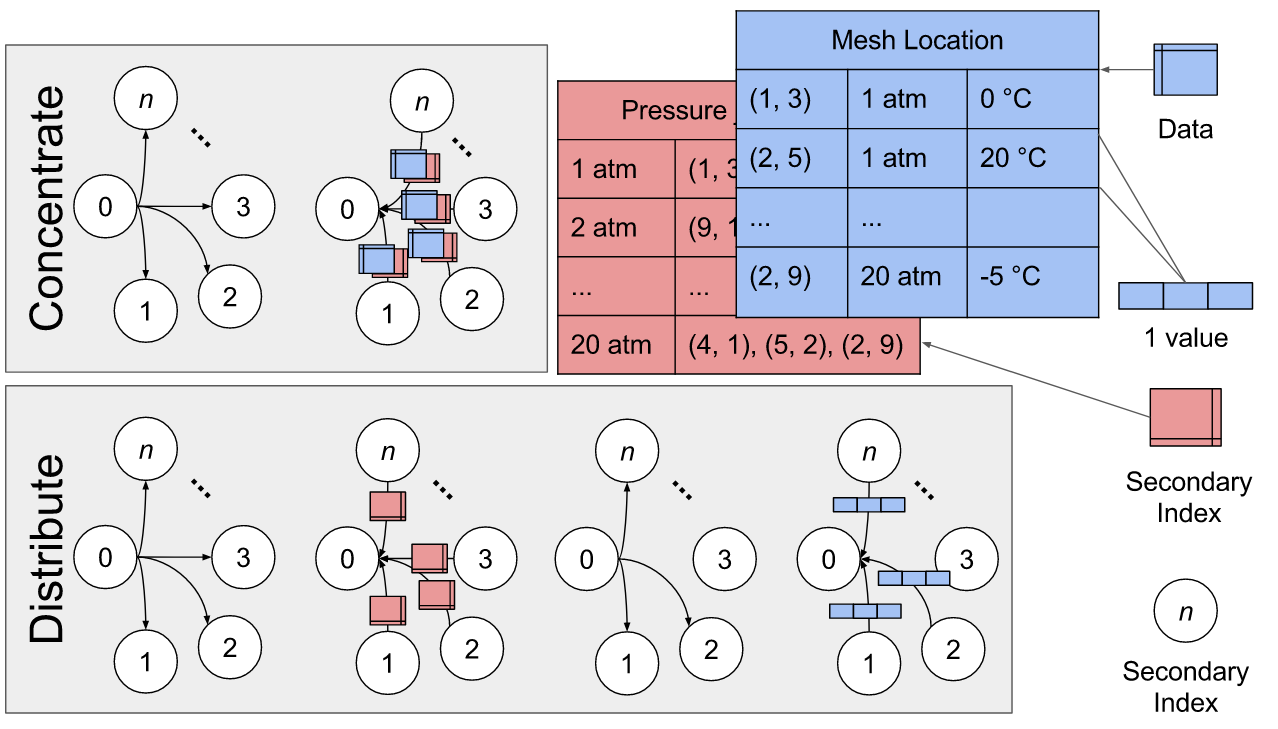
\includegraphics[width=19pc,angle=0]{figures/example.png}\\
\appendcaption{A1}{Balancing for distribution takes more RPCs while migrating for concentration risk of overloading the client.}
\end{figure}


